\documentclass[11pt]{article}
\usepackage{amsmath,amssymb,amsmath,amsthm,amsfonts}
\usepackage{latexsym,graphicx}
\usepackage{fullpage,color}
\usepackage{url}
\usepackage[pdftex,bookmarks,colorlinks=true,citecolor=blue]{hyperref}
\usepackage{natbib}
\usepackage{graphicx,subfigure}
\usepackage{algorithm}
\usepackage{algorithmic}
\usepackage{listings}
\usepackage{xcolor}
\usepackage{framed}
\usepackage{color}

% \colorlet{shadecolor}{orange!15}
\colorlet{NextBlue}{orange!15!green!50!blue!75}

\numberwithin{equation}{section}

\pagestyle{plain}

\setlength{\oddsidemargin}{0in}
\setlength{\topmargin}{0in}
\setlength{\textwidth}{6.5in}
\setlength{\textheight}{8.5in}

\newtheorem{fact}{Fact}[section]
\newtheorem{question}{Question}[section]
\newtheorem{lemma}{Lemma}[section]
\newtheorem{theorem}[lemma]{Theorem}
\newtheorem{assumption}[lemma]{Assumption}
\newtheorem{corollary}[lemma]{Corollary}
\newtheorem{prop}[lemma]{Proposition}
\newtheorem{claim}{Claim}[section]
\newtheorem{remark}{Remark}[section]
\newtheorem{definition}{Definition}[section]
\newtheorem{prob}{Problem}[section]
\newtheorem{conjecture}{Conjecture}[section]
\newtheorem{property}{Property}[section]

\def\A{{\bf A}}
\def\a{{\bf a}}
\def\B{{\bf B}}
\def\bb{{\bf b}}
\def\C{{\bf C}}
\def\c{{\bf c}}
\def\D{{\bf D}}
\def\d{{\bf d}}
\def\E{{\bf E}}
\def\e{{\bf e}}
\def\F{{\bf F}}
\def\f{{\bf f}}
\def\g{{\bf g}}
\def\h{{\bf h}}
\def\G{{\bf G}}
\def\H{{\bf H}}
\def\I{{\bf I}}
\def\K{{\bf K}}
\def\k{{\bf k}}
\def\LL{{\bf L}}
\def\M{{\bf M}}
\def\m{{\bf m}}
\def\N{{\bf N}}
\def\n{{\bf n}}
\def\PP{{\bf P}}
\def\pp{{\bf p}}
\def\Q{{\bf Q}}
\def\q{{\bf q}}
\def\R{{\bf R}}
\def\rr{{\bf r}}
\def\S{{\bf S}}
\def\s{{\bf s}}
\def\T{{\bf T}}
\def\tt{{\bf t}}
\def\U{{\bf U}}
\def\u{{\bf u}}
\def\V{{\bf V}}
\def\v{{\bf v}}
\def\W{{\bf W}}
\def\w{{\bf w}}
\def\X{{\bf X}}
\def\x{{\bf x}}
\def\Y{{\bf Y}}
\def\y{{\bf y}}
\def\Z{{\bf Z}}
\def\z{{\bf z}}
\def\0{{\bf 0}}
\def\1{{\bf 1}}



\def\AM{{\mathcal A}}
\def\CM{{\mathcal C}}
\def\DM{{\mathcal D}}
\def\EM{{\mathcal E}}
\def\GM{{\mathcal G}}
\def\FM{{\mathcal F}}
\def\IM{{\mathcal I}}
\def\JM{{\mathcal J}}
\def\KM{{\mathcal K}}
\def\LM{{\mathcal L}}
\def\NM{{\mathcal N}}
\def\OM{{\mathcal O}}
\def\PM{{\mathcal P}}
\def\SM{{\mathcal S}}
\def\TM{{\mathcal T}}
\def\UM{{\mathcal U}}
\def\VM{{\mathcal V}}
\def\WM{{\mathcal W}}
\def\XM{{\mathcal X}}
\def\YM{{\mathcal Y}}
\def\RB{{\mathbb R}}
\def\RBmn{{\RB^{m\times n}}}
\def\EB{{\mathbb E}}
\def\PB{{\mathbb P}}

\def\TX{\tilde{\bf X}}
\def\TA{\tilde{\bf A}}
\def\tx{\tilde{\bf x}}
\def\ty{\tilde{\bf y}}
\def\TZ{\tilde{\bf Z}}
\def\tz{\tilde{\bf z}}
\def\hd{\hat{d}}
\def\HD{\hat{\bf D}}
\def\hx{\hat{\bf x}}
\def\nysA{{\tilde{\A}_c^{\textrm{nys}}}}

\def\alp{\mbox{\boldmath$\alpha$\unboldmath}}
\def\bet{\mbox{\boldmath$\beta$\unboldmath}}
\def\epsi{\mbox{\boldmath$\epsilon$\unboldmath}}
\def\etab{\mbox{\boldmath$\eta$\unboldmath}}
\def\ph{\mbox{\boldmath$\phi$\unboldmath}}
\def\pii{\mbox{\boldmath$\pi$\unboldmath}}
\def\Ph{\mbox{\boldmath$\Phi$\unboldmath}}
\def\Ps{\mbox{\boldmath$\Psi$\unboldmath}}
\def\ps{\mbox{\boldmath$\psi$\unboldmath}}
\def\tha{\mbox{\boldmath$\theta$\unboldmath}}
\def\Tha{\mbox{\boldmath$\Theta$\unboldmath}}
\def\muu{\mbox{\boldmath$\mu$\unboldmath}}
\def\Si{\mbox{\boldmath$\Sigma$\unboldmath}}
\def\si{\mbox{\boldmath$\sigma$\unboldmath}}
\def\Gam{\mbox{\boldmath$\Gamma$\unboldmath}}
\def\Lam{\mbox{\boldmath$\Lambda$\unboldmath}}
\def\De{\mbox{\boldmath$\Delta$\unboldmath}}
\def\Ome{\mbox{\boldmath$\Omega$\unboldmath}}
\def\Pii{\mbox{\boldmath$\Pi$\unboldmath}}
\def\varepsi{\mbox{\boldmath$\varepsilon$\unboldmath}}
\newcommand{\ti}[1]{\tilde{#1}}
\def\Ncal{\mathcal{N}}
\def\argmax{\mathop{\rm argmax}}
\def\argmin{\mathop{\rm argmin}}

\def\ALG{{\AM_{\textrm{col}}}}

\def\mean{\mathsf{mean}}
\def\std{\mathsf{std}}
\def\bias{\mathsf{bias}}
\def\var{\mathsf{var}}
\def\sgn{\mathsf{sgn}}
\def\tr{\mathsf{tr}}
\def\rk{\mathrm{rank}}
\def\nnz{\mathsf{nnz}}
\def\poly{\mathrm{poly}}
\def\diag{\mathsf{diag}}
\def\Diag{\mathsf{Diag}}
\def\const{\mathrm{Const}}
\def\st{\mathsf{s.t.}}
\def\vect{\mathsf{vec}}
\def\sech{\mathrm{sech}}
\def\sigmoid{\mathsf{sigmoid}}

\newcommand{\red}[1]{{\color{red}#1}}



\def\argmax{\mathop{\rm argmax}}
\def\argmin{\mathop{\rm argmin}}

\newenvironment{note}[1]{\medskip\noindent \textbf{#1:}}%
        {\medskip}


\newcommand{\etal}{{\em et al.}\ }
\newcommand{\assign}{\leftarrow}
\newcommand{\eps}{\epsilon}

\newcommand{\opt}{\textrm{\sc OPT}}
\newcommand{\script}[1]{\mathcal{#1}}
\newcommand{\ceil}[1]{\lceil #1 \rceil}
\newcommand{\floor}[1]{\lfloor #1 \rfloor}



\lstset{ %
extendedchars=false,            % Shutdown no-ASCII compatible
language=Python,                % choose the language of the code
xleftmargin=1em,
xrightmargin=1em,
basicstyle=\footnotesize,    % the size of the fonts that are used for the code
tabsize=3,                            % sets default tabsize to 3 spaces
numbers=left,                   % where to put the line-numbers
numberstyle=\tiny,              % the size of the fonts that are used for the line-numbers
stepnumber=1,                   % the step between two line-numbers. If it's 1 each line
                                % will be numbered
numbersep=5pt,                  % how far the line-numbers are from the code   %
keywordstyle=\color[rgb]{0,0,1},                % keywords
commentstyle=\color[rgb]{0.133,0.545,0.133},    % comments
stringstyle=\color[rgb]{0.627,0.126,0.941},      % strings
backgroundcolor=\color{white}, % choose the background color. You must add \usepackage{color}
showspaces=false,               % show spaces adding particular underscores
showstringspaces=false,         % underline spaces within strings
showtabs=false,                 % show tabs within strings adding particular underscores
frame=single,                 % adds a frame around the code
%captionpos=b,                   % sets the caption-position to bottom
breaklines=true,                % sets automatic line breaking
breakatwhitespace=false,        % sets if automatic breaks should only happen at whitespace
%title=\lstname,                 % show the filename of files included with \lstinputlisting;
%                                % also try caption instead of title
mathescape=true,escapechar=?    % escape to latex with ?..?
escapeinside={\%*}{*)},         % if you want to add a comment within your code
%columns=fixed,                  % nice spacing
%morestring=[m]',                % strings
%morekeywords={%,...},%          % if you want to add more keywords to the set
%    break,case,catch,continue,elseif,else,end,for,function,global,%
%    if,otherwise,persistent,return,switch,try,while,...},%
}


\begin{document}

%\setlength{\fboxrule}{.5mm}\setlength{\fboxsep}{1.2mm}
%\newlength{\boxlength}\setlength{\boxlength}{\textwidth}
%\addtolength{\boxlength}{-4mm}


\title{Property Inference Attacks on Fully Connected Neural Networks using Permutation Invariant Representations}

\author{\textbf{Karan Ganju \etal} \\ University of Illinois at Urbana-Champaign, USA}

%\date{ }

\maketitle

\begin{abstract}
% This lecture note describes synchronous parallel accelerated gradient descent (AGD) for empirical risk minimization ERM.
% We first describe AGD for solving ERM.
% We then show how to parallelize AGD; in particular, we assume there is a central parameter server and the data are partitioned among the worker nodes.
% We finally use Python to write a simulator that mimics synchronous parallel AGD.
This paper describes property inference attacks on fully connected neural networks.

Sharing the learned models is becoming popular. However, in addition to the prediction properties the model producer aims to share, there is also a risk that the model consumer can infer {\color{blue}\textit{other properties}} of the training data the model producer \textit{did not intend to share}.(e.g. the environment in which the data was produced, the fraction of the data that comes from a certain class.) This is a white box attack.

\end{abstract}

\section{Property inference attack} 

\begin{itemize}
    \item meta-classifier ($\mathbb M \mathbb C$): to classify the\textit{ target classifier is ($C_x$)} wheter it has a property $P$ or not.
    \item a set of \textit{shadow classifier}($C_1, C_2, \cdots ,C_n$): trained on the same task as the target classifier. Each classifier is trained on a dataset($D_1, D_2, \cdots, D_n$) similar to that of the target classifier but constructed explicitly to either have or not have the property $P$.
    \item The input of meta-classifier: the parameters of the shadow classifiers
\end{itemize}

\begin{figure}[!h]
	\centering
	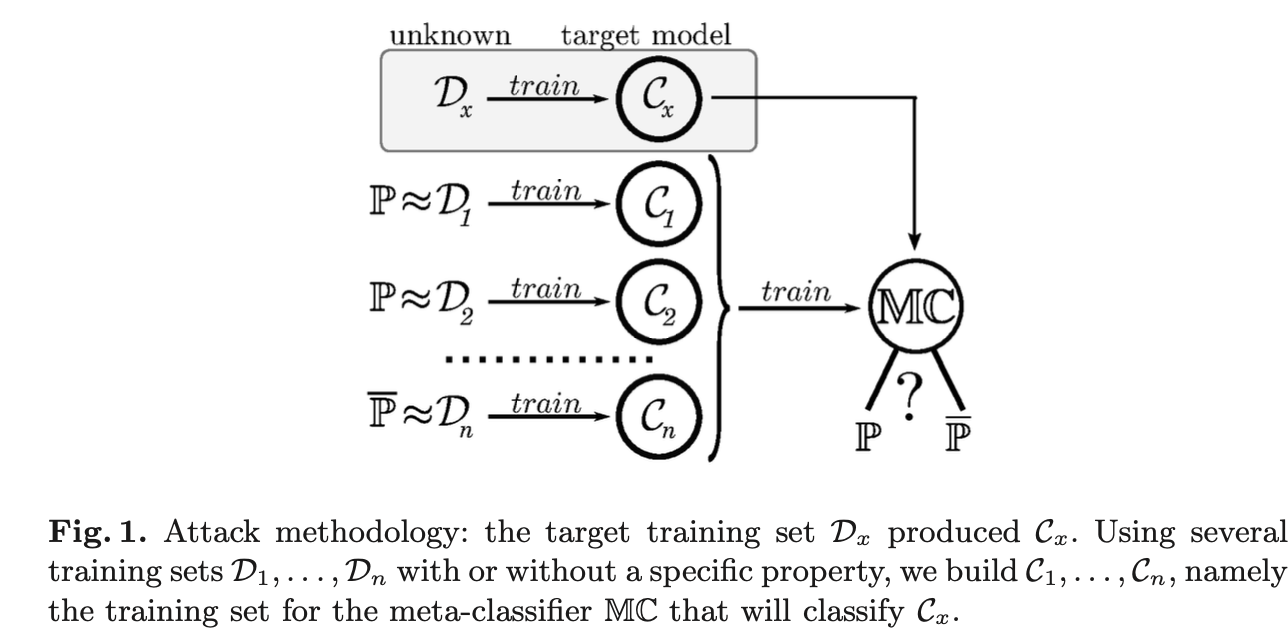
\includegraphics[width=12cm]{figures/property_inference_model.png}
% 	\caption{Illustration of parallel AGD.}
	\label{fig:property inference model}
\end{figure}



\section{The difficulties of applying this kind attack to deep neural networks}

\begin{itemize}
    \item the models are often very complex and have more than thousands of parameters, so it is very hard to train a meta-classifier.
    \item The invariance property is challenging for meta-classifier to learn.(invariance property: applying an arbitrary permutation to each hidden layer of a FCNN and adjusting the weights correspondingly results in an equivalent FCNN).
    \item the number of such equivalent networks grows super-exponentially in the number of nodes.
\end{itemize}

An example of permutation equivalent neural networks.

\begin{figure}[!h]
	\centering
	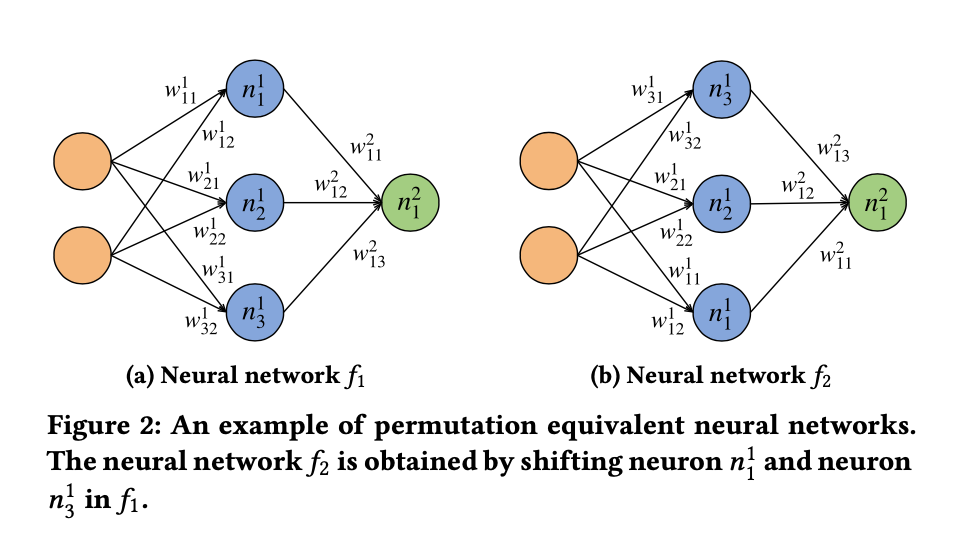
\includegraphics[width=10cm]{figures/permutation_example.png}
% 	\caption{Illustration of parallel AGD.}
	\label{fig:property inference model}
\end{figure}

Experiment to show these equivalents are found in the wild.

input: a single number
output: positive or negative
hidden layer: one hidden layer with 2 nodes.

The distribution of two weights of hidden layer:

\begin{figure}[!h]
	\centering
	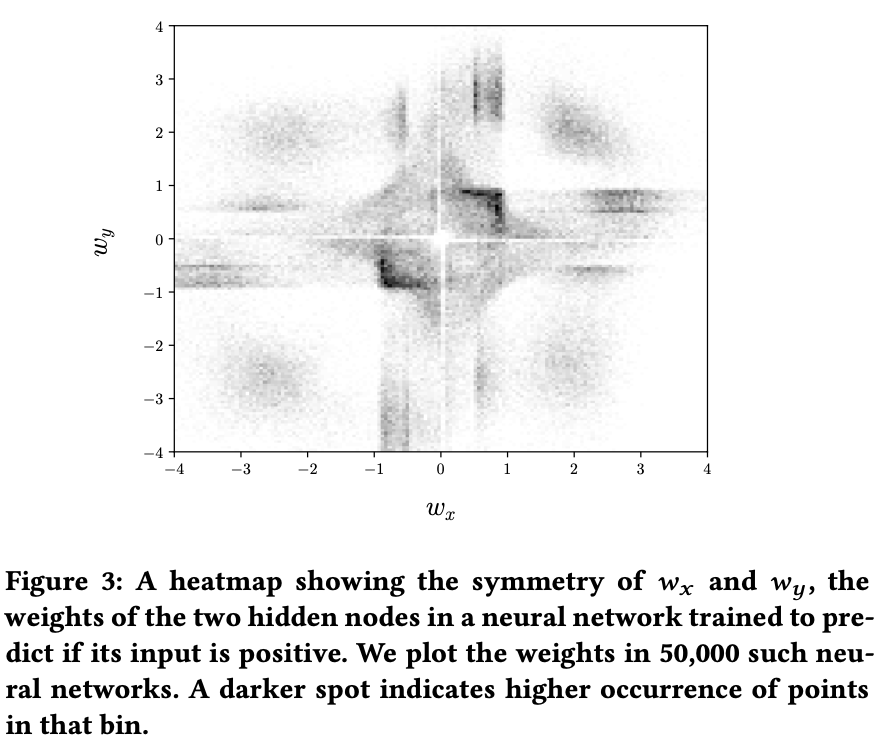
\includegraphics[width=8cm]{figures/two_hidden_distribution.png}
% 	\caption{Illustration of parallel AGD.}
	\label{fig:property inference model}
\end{figure}

The plot is symmetric along the $Y = X$ line. This means that for each weight pair $(w_x, w_y)$, there is also a pair $(w_y, w_x)$

\section{Ways to solve the difficulties above:}
\begin{enumerate}
    \item arrange the FCNN into a canonical form (sorting neurons in each layer)
    \item represent each layer of a FCNN as a set rather than an ordered vector.(DeepSets architecture. Reduce the number of parameters in the meta-classifier, making it easier to train)
\end{enumerate}

\subsection{Neuron Sorting}

Similar to pre-processing step of face recognition.

\begin{itemize}
    \item Example: A facial recognition model does not take rotation of faces into account. The images are aligned in a canonical pose.
\end{itemize}

Fact of FCNN: we can perform node permutations on hidden layers of a fully connected neural network without changing the function that it represents.

To ensure that all permutation equivalents have the same representation: apply a permutation that imposes a canonical ordering(or sorting) for each of the hidden layers.

The process to take in a classifier $f$ and returns its sorted feature representation $F$.

\begin{enumerate}
    \item For each layer: computer a metric for each of its nodes.(e.g. magnitude of the sum of weights)
    \item Find a permutation that sorts these metrics
    \item Apply this permutation as a node permutation to the same layer and add its sorted flattened weights and biases to $F$
    \item Move to next layer and repeat
\end{enumerate}

One advantage of this approach: after sorting, the feature representation of the neural network is still a flattened vector, which can be used with generic machine learning algorithms, such as decision tree or neural networks as the meta-classifier.


\subsection{Set-Based Representation}

Solve this task through a more intelligent design of the meta-classifier instead. 

Represent a neural network layer as a set of neurons not a flattened vector of nodes with the aid of DeepSets.

DeepSets consists of two parts(two neural networks, or two functions):

\begin{equation*}
    y = f(X) = \rho\left(\sum_{x \in X}\phi(x)\right)
\end{equation*}

$X:$ a set

$\phi:$ to obtain an element-level representation(or proposed feature)

$\rho:$ to obtain a final prediction (or output) for the set.


\begin{figure}[!h]
	\centering
	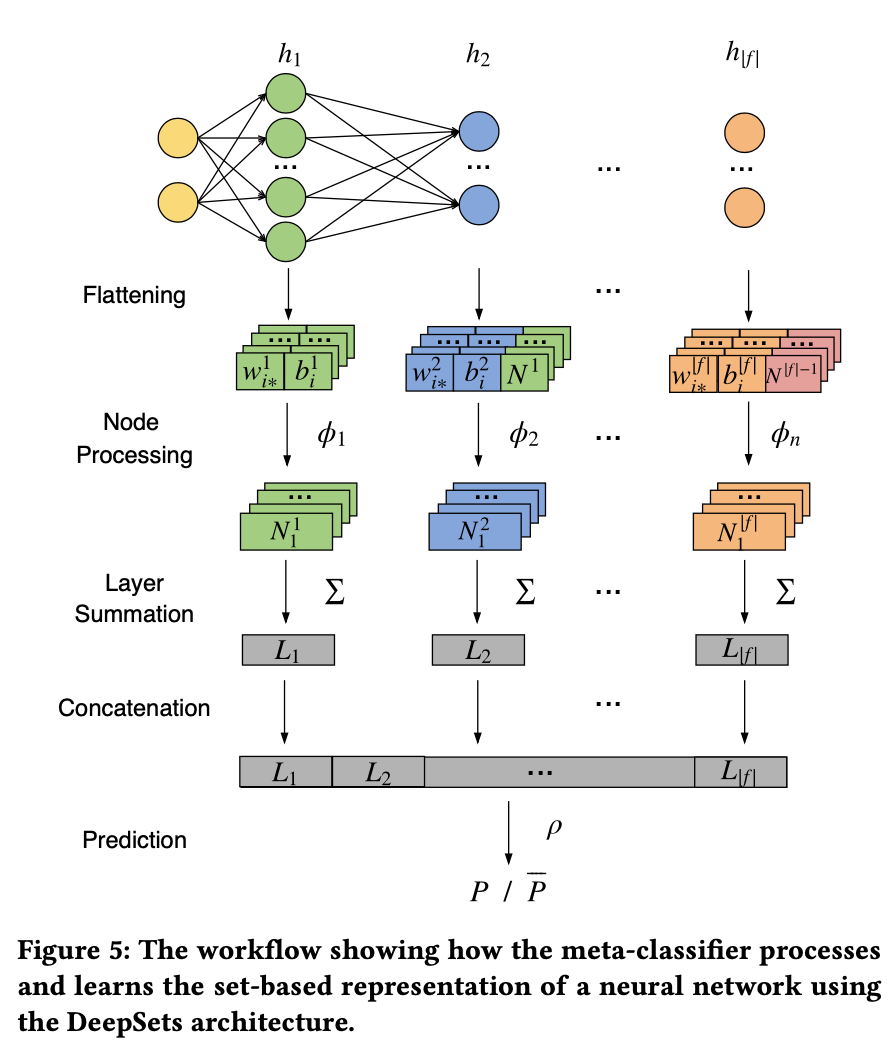
\includegraphics[width=12cm]{figures/Set_model.png}
% 	\caption{Illustration of parallel AGD.}
	\label{fig:property inference model}
\end{figure}


\section{Evaluation}

\begin{figure}[H]
	\centering
	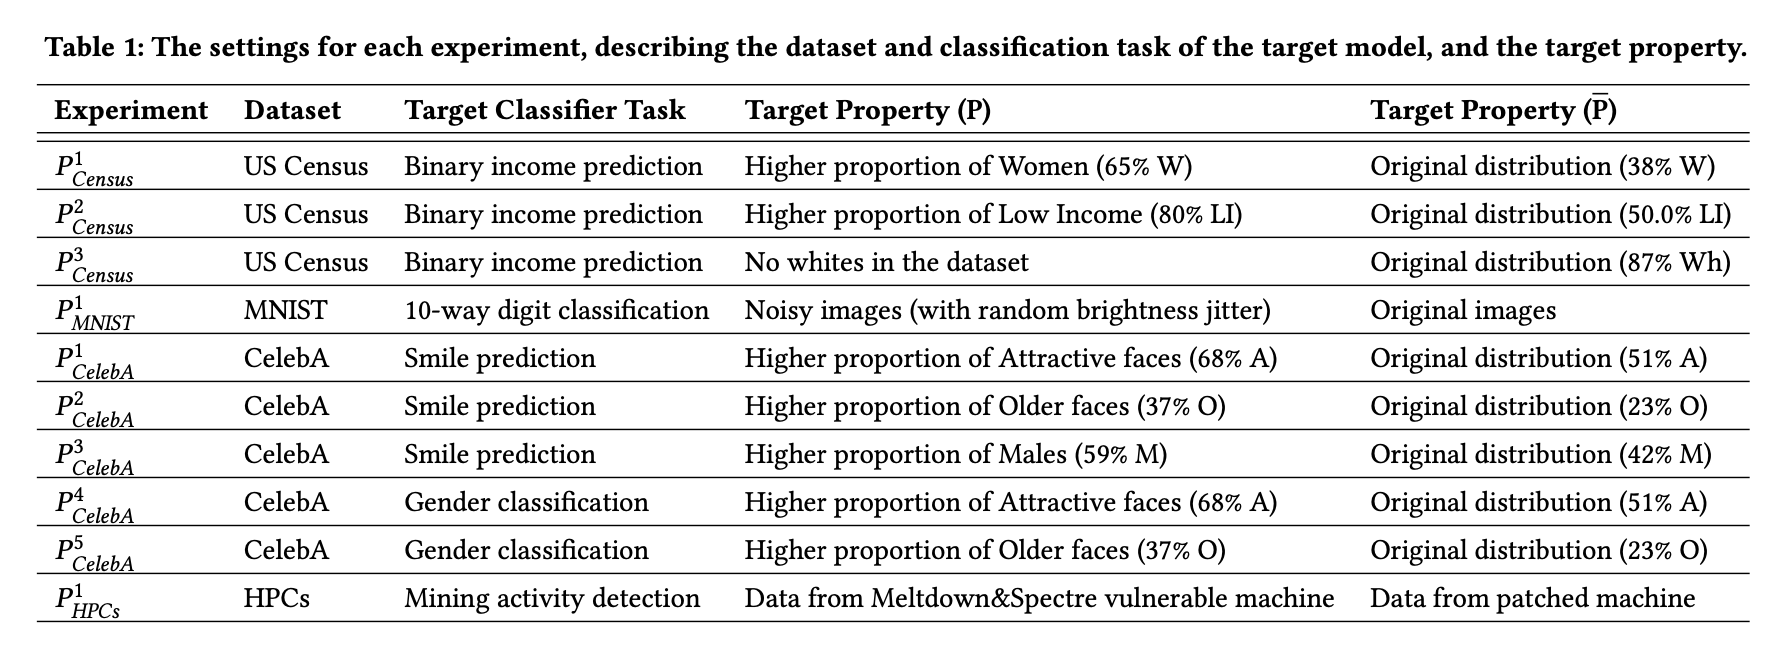
\includegraphics[width=15cm]{figures/Data_setup.png}
% 	\caption{Illustration of parallel AGD.}
	\label{fig:property inference model}
\end{figure}

\begin{figure}[H]
	\centering
	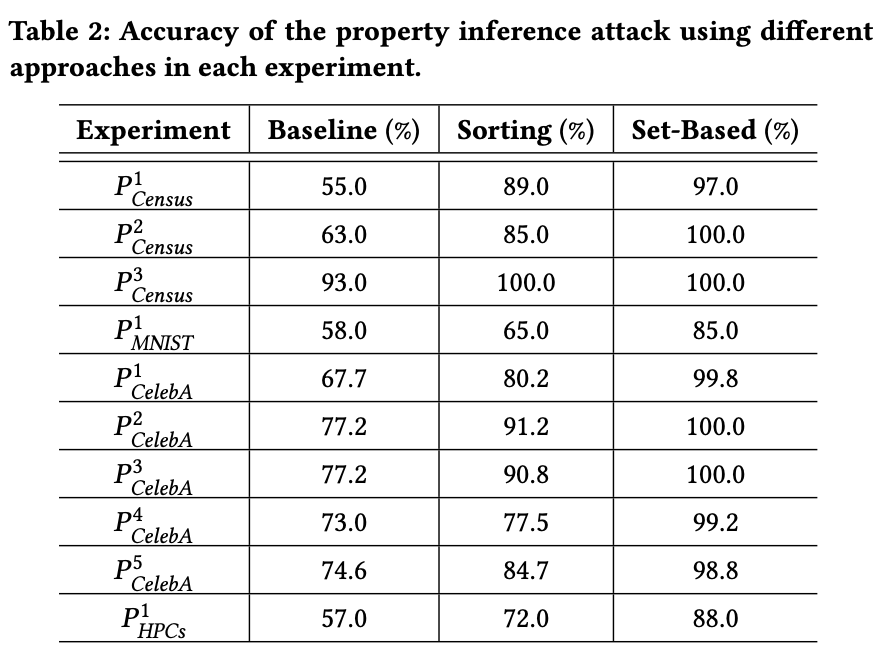
\includegraphics[width=12cm]{figures/Accuracy_diff_approches.png}
% 	\caption{Illustration of parallel AGD.}
	\label{fig:property inference model}
\end{figure}

\begin{figure}[H]
	\centering
	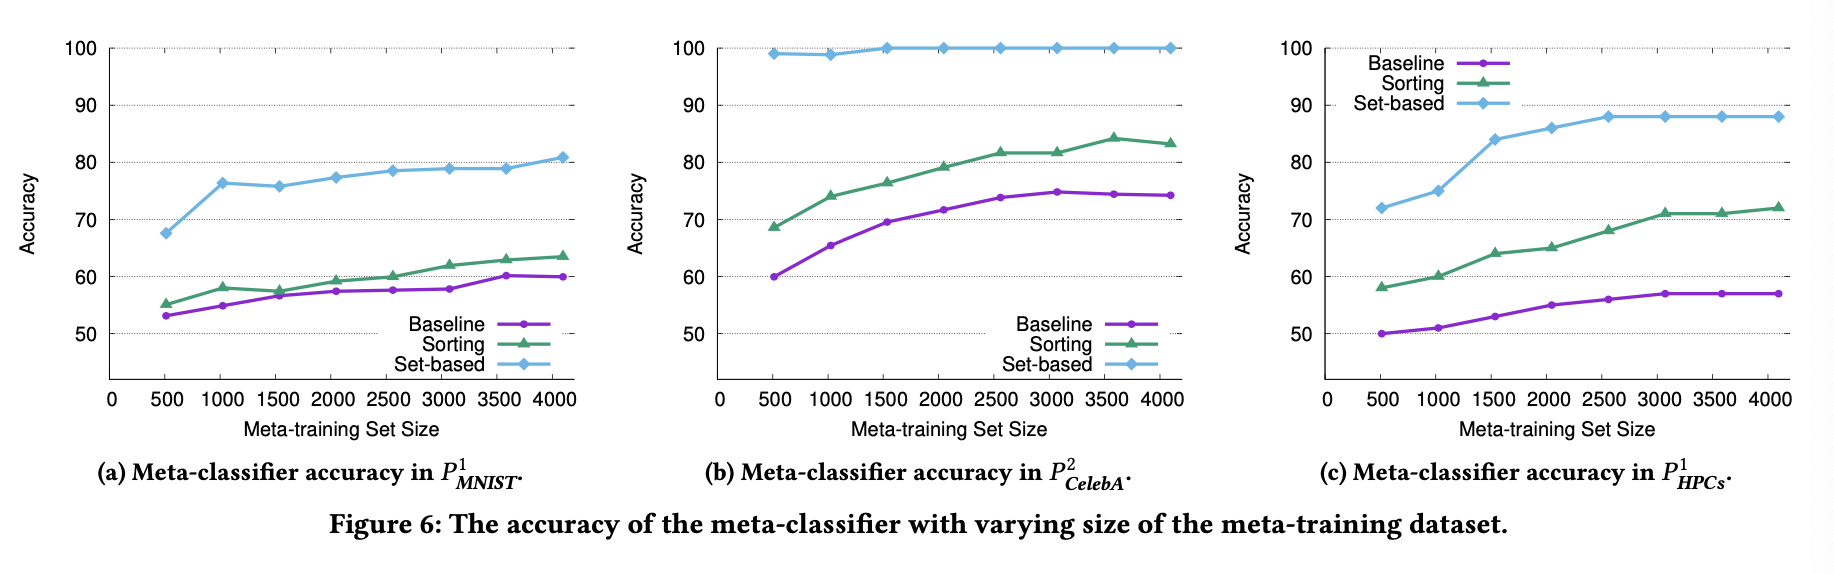
\includegraphics[width=15cm]{figures/efficiency.png}
% 	\caption{Illustration of parallel AGD.}
	\label{fig:property inference model}
\end{figure}

\begin{figure}[H]
	\centering
	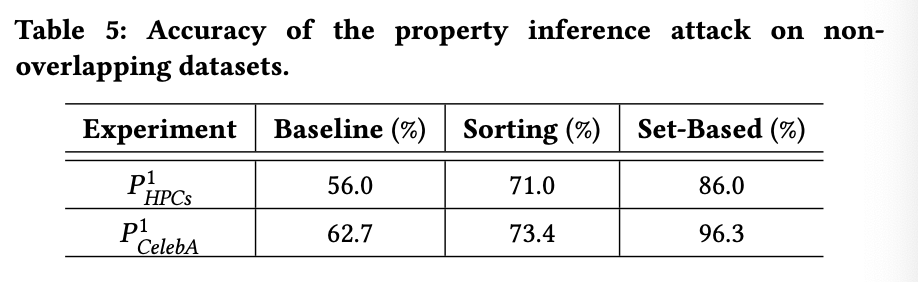
\includegraphics[width=15cm]{figures/non_overlapping datasets.png}
% 	\caption{Illustration of parallel AGD.}
	\label{fig:property inference model}
\end{figure}


\section{limitations and future work}

\begin{enumerate}
    \item Other types of neural networks
    \begin{itemize}
        \item mainly focus on fully connected networks
        \item can perform property inference just using the FC layers trained on the output of a pre-trained convolutional model.
        \item believe it is possible to apply this approach to other types of NN.
    \end{itemize}
    \item over-fitting
    \begin{itemize}
        \item overfitting is a major factor that causes a model to be vulnerable to membership inference attacks.
        \item it is not clear whether overfitting of target classifiers has any role in the property inference attack.
        \item study the relationship between overfitting and property inference in the future
    \end{itemize}
    \item membership inference
    \begin{itemize}
        \item plan to study the relationship between membership inference and property inference in the future
    \end{itemize}
    \item Multi-label or Regression based Properties.
    \begin{itemize}
        \item only study binary-class property inference
        \item extend the approach for multi-class and regression tasks in the future
    \end{itemize}
    \item Generating Training Data for Shadow Models
    \begin{itemize}
        \item the attacker may have no access to similar training dataset
        \item the attacker may have no knowledge of the dataset generation technique
    \end{itemize}
\end{enumerate}

\section{Possible Defenses}

the model producer could manipulate the parameters of the model directly or indirectly to make it "different" from the shadow models.

\begin{enumerate}
    \item Using Node Multiplicative Transformations
    \begin{itemize}
        \item multiplying the weights and bias of the neuron by some constant and dividing the weights connecting it to the next layer by the same constant
        \item the attack accuracy of our approaches decreases as we increase the fraction of perturbed neurons
        \item can only be used by deep neural networks that use ReLU or LeakyReLU as activation function
    \end{itemize}
    \item Adding Noisy Data to the Training Set
    \begin{itemize}
        \item flipping the labels of some training samples
        \item might hamper the effectiveness
    \end{itemize}
    \item Encoding Arbitrary Information
    \begin{itemize}
        \item Deep neural networks have huge capacity for “memorizing” arbitrary information
        \item encode some arbitrary information in the model, making the parameters look different from those of the shadow classifiers
    \end{itemize}
\end{enumerate}

\bibliographystyle{plain}

%\markboth{\bibname}{\bibname}
% \bibliography{bib/decentralized,bib/distributed,bib/system}
\bibliography{bib/decentralized,bib/distributed,bib/system,bib/poison}

\end{document}
